\specialchapter{\texorpdfstring{图版 IV. \(D_{l}\) 型根系（\(l \geqslant 3\)）}{图版 IV. D\_l 型根系 (l >= 3)}}

\begin{enumerate}
\def\labelenumi{(\Roman{enumi})}
\tightlist
\item
  \(V = E = R^{l}\) 。根：\(\pm\varepsilon_{i}\pm\varepsilon_{j}(1\leqslant i<j\leqslant l)\)；（ \(\varepsilon_{i}\) ）是 \(R^{l}\) 的标准基。根的数目：\(n = 2l(l - 1)\) 。
\end{enumerate}

\begin{enumerate}
\def\labelenumi{(\Roman{enumi})}
\setcounter{enumi}{1}
\tightlist
\item
  基：\(\alpha_{1} = \varepsilon_{1} - \varepsilon_{2},\alpha_{2} = \varepsilon_{2} - \varepsilon_{3},\ldots ,\alpha_{l - 1} = \varepsilon_{l - 1} - \varepsilon_{l},\alpha_{l} = \varepsilon_{l - 1} + \varepsilon_{l}\) 。正根：
\end{enumerate}

\[
\varepsilon_ {i} - \varepsilon_ {j} = \sum_ {i <   k <   j} \alpha_ {k} (1 \leqslant i <   j \leqslant l).
\]

\[
\varepsilon_ {i} + \varepsilon_ {l} = \sum_ {i \leqslant k \leqslant l - 2} \alpha_ {k} + \alpha_ {l} (1 \leqslant i <   l),
\]

\[
\varepsilon_ {i} + \varepsilon_ {j} = \sum_ {i \leqslant k <   j} \alpha_ {k} + 2 \sum_ {j \leqslant k <   l - 1} \alpha_ {k} + \alpha_ {l - 1} + \alpha_ {l} (1 \leqslant i <   j <   l).
\]

\begin{enumerate}
\def\labelenumi{(\Roman{enumi})}
\setcounter{enumi}{2}
\item
  Coxeter 数：\(h = 2l - 2\) 。
\item
  最高根：
\end{enumerate}

\[
\tilde {\alpha} = \varepsilon_ {1} + \varepsilon_ {2} = \alpha_ {1} + 2 \alpha_ {2} + \dots + 2 \alpha_ {l - 2} + \alpha_ {l - 1} + \alpha_ {l}.
\]

有 \(\tilde{\alpha} = \omega_2 + \omega_3\)，当 \(l = 3\) 时；有 \(\tilde{\alpha} = \omega_2\)，当 \(l \geqslant 4\) 时。

扩展 Dynkin 图（l ≥ 4）：

\pandocbounded{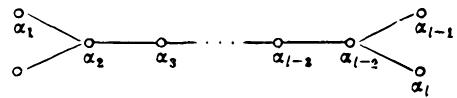
\includegraphics[keepaspectratio]{images/part002_b62b20f1.jpg}}

\begin{enumerate}
\def\labelenumi{(\Alph{enumi})}
\setcounter{enumi}{21}
\tightlist
\item
  \(R^{\prime} = R.\)
\end{enumerate}

\[
\Phi_ {R} (x, y) = \frac {(x | y)}{4 (l - 1)}, \quad \gamma (R) = 4 (l - 1) ^ {2}.
\]

\begin{enumerate}
\def\labelenumi{(\Roman{enumi})}
\setcounter{enumi}{5}
\tightlist
\item
  基本权：
\end{enumerate}

\[
\begin{array}{r l} \omega_ {i} & = \varepsilon_ {1} + \varepsilon_ {2} + \dots + \varepsilon_ {i} (1 \leqslant i \leqslant l - 2) \\ & = \alpha_ {1} + 2 \alpha_ {2} + \dots + (i - 1) \alpha_ {i - 1} + i (\alpha_ {i} + \alpha_ {i + 1} + \dots + \alpha_ {l - 2}) \\ & \quad + \frac {1}{2} i (\alpha_ {l - 1} + \alpha_ {l}) \\ \omega_ {l - 1} & = \frac {1}{2} (\varepsilon_ {1} + \varepsilon_ {2} + \dots + \varepsilon_ {l - 2} + \varepsilon_ {l - 1} - \varepsilon_ {l}) \\ & = \frac {1}{2} (\alpha_ {1} + 2 \alpha_ {2} + \dots + (l - 2) \alpha_ {l - 2} + \frac {1}{2} l \alpha_ {l - 1} + \frac {1}{2} (l - 2) \alpha_ {l}) \\ \omega_ {l} & = \frac {1}{2} (\varepsilon_ {1} + \varepsilon_ {2} + \dots + \varepsilon_ {l - 2} + \varepsilon_ {l - 1} + \varepsilon_ {l}) \\ & = \frac {1}{2} (\alpha_ {1} + 2 \alpha_ {2} + \dots + (l - 2) \alpha_ {l - 2} + \frac {1}{2} (l - 2) \alpha_ {l - 1} + \frac {1}{2} l \alpha_ {l}). \end{array}
\]

\begin{enumerate}
\def\labelenumi{(\Roman{enumi})}
\setcounter{enumi}{6}
\tightlist
\item
  正根之和：
\end{enumerate}

\[
\begin{array}{r l} 2 \rho & = 2 (l - 1) \varepsilon_ {1} + 2 (l - 2) \varepsilon_ {2} + \dots + 2 \varepsilon_ {l - 1} \\ & = 2 (l - 1) \alpha_ {1} + 2 (2 l - 3) \alpha_ {2} + \dots + 2 (i l - \frac {i (i + 1)}{2}) \alpha_ {i} + \dots \\ & \qquad \dots + \frac {l (l - 1)}{2} (\alpha_ {l - 1} + \alpha_ {l}). \end{array}
\]

\begin{enumerate}
\def\labelenumi{(\Roman{enumi})}
\setcounter{enumi}{7}
\tightlist
\item
  Q(R)：坐标为整数且和为偶数的点集。
\end{enumerate}

\[
\mathrm{P} (\mathrm{R}) = \bigoplus_ {i = 1} ^ {l} \mathbf {Z} \varepsilon_ {i} + \mathbf {Z} \left(\frac {1}{2} \sum_ {i = 1} ^ {l} \varepsilon_ {i}\right).
\]

l 为奇数时：\(\mathrm{P}(\mathrm{R})/\mathrm{Q}(\mathrm{R})\) 同构于 Z/4Z，由 \(\omega_{l}\) 的像生成；有 \(\omega_{1} \equiv 2\omega_{l}\) 和 \(\omega_{l-1} \equiv 3\omega_{l} \mod Q(\mathrm{R})\)。l 为偶数时：\(\mathrm{P}(\mathrm{R})/\mathrm{Q}(\mathrm{R})\) 同构于 \((\mathbf{Z}/2\mathbf{Z}) \times (\mathbf{Z}/2\mathbf{Z})\)；阶为 2 的三个元素是 \(\omega_{1}, \omega_{l-1}\) 和 \(\omega_{l}\) 的像。连接指标：4。

\begin{enumerate}
\def\labelenumi{(\Roman{enumi})}
\setcounter{enumi}{8}
\item
  指数：1, 3, 5, \ldots, 2l - 5, 2l - 3, l - 1（最后一个在 l 为偶数时出现两次，在 l 为奇数时出现一次）。
\item
  W(R) 是群 \(S_{l}\)（通过对 \(\varepsilon_{i}\) 进行置换作用）与群 \((\mathbf{Z}/2\mathbf{Z})^{l-1}\)（通过 \(\varepsilon_{i} \mapsto (\pm1)_{i}\varepsilon_{i}\) 作用，并满足 \(\prod_{i}(\pm1)_{i} = 1\)）的半直积。其阶为 \(2^{l-1}.l!\)
\item
  \(l \neq 4\)：A(R)/W(R) = Z/2Z 通过交换节点 \(\alpha_{l-1}\) 和 \(\alpha_l\) 作用于 Dynkin 图。\(l = 4\)：A(R)/W(R) = \(\mathfrak{S}_3\)，通过置换节点 \(\alpha_1, \alpha_3\) 和 \(\alpha_4\) 作用于 Dynkin 图。\(w_0 = -1\) 在 \(l\) 为偶数时成立；\(w_0 = -\varepsilon\) 在 \(l\) 为奇数时成立，其中 \(\varepsilon\) 是交换 \(\alpha_{l-1}\) 与 \(\alpha_l\) 并固定其余 \(\alpha_i\) 的自同构。
\item
  \(\mathrm{P}(\mathbb{R}^{-}) / \mathrm{Q}(\mathbb{R}^{-}) = \mathrm{P}(\mathbb{R}) / \mathrm{Q}(\mathbb{R})\) 在扩展 Dynkin 图上的作用：\(l\) 为奇数时，\(\omega_l\) 将 \(\alpha_0\) 变为 \(\alpha_1\)，将 \(\alpha_l\) 变为 \(\alpha_1\)，将 \(\alpha_1\) 变为 \(\alpha_{l-1}\)，并将 \(\alpha_{l-1}\) 变为 \(\alpha_0\)；它交换 \(\alpha_j\) 和 \(\alpha_{l-j}\)，其中 \(2 \leqslant j \leqslant l - 2\)。\(l\) 为偶数时，\(\omega_l\)（分别为 \(\omega_{l-1}\)）交换 \(\alpha_0\) 和 \(\alpha_l\)（分别为 \(\alpha_0\) 和 \(\alpha_{l-1}\)）、\(\alpha_1\) 和 \(\alpha_{l-1}\)（分别为 \(\alpha_1\) 和 \(\alpha_l\)），并交换 \(\alpha_j\) 和 \(\alpha_{l-j}\)，其中 \(2 \leqslant j \leqslant l - 2\)。
\end{enumerate}

\[
\left( \begin{array}{c c c c c c c} 2 & - 1 & \dots & 0 & 0 & 0 & 0 \\ - 1 & 2 & \dots & 0 & 0 & 0 & 0 \\ \vdots & \vdots & \ddots & \vdots & \vdots & \vdots & \vdots \\ 0 & 0 & \dots & 2 & - 1 & 0 & 0 \\ 0 & 0 & \dots & - 1 & 2 & - 1 & - 1 \\ 0 & 0 & \dots & 0 & - 1 & 2 & 0 \\ 0 & 0 & \dots & 0 & - 1 & 0 & 2 \end{array} \right)
\]

\begin{enumerate}
\def\labelenumi{(\Roman{enumi})}
\setcounter{enumi}{12}
\tightlist
\item
  Cartan 矩阵 \((l\times l)\) ：
\end{enumerate}

